\documentclass[12pt]{article}
\usepackage{graphicx}
\usepackage{epstopdf}
%
% Title[Enter title of the experiment here]
\title{EE230:experiment No.5\\
Opamp circuits-3}

% Author[Enter details of author here]
\author{Mudavtah vishnuvardhan,200070044}

% begin the document.
\begin{document}

% make a title page.[this creates title page]
\maketitle


\section{Overview of the experiment} %[This segment creates Section as seen in document]

\subsection{Aim of the experiment}%[This segment creates sebsections under the same section]
To simulate the following circuits using NGSPICE
and compare the results with experimental observations:\\
1. Photodiode application circuit using op-amp LM324\\
2. 3 op-amp based Instrumentation Amplifier\\


\subsection{Methods}

The simulating software used is Ngspice.
We used the provided model files for diode and op-amp. 

\section{Circuit Design}
\subsection{Photodiode Application Circuit}
\\
\begin{figure}[h!]
\centering
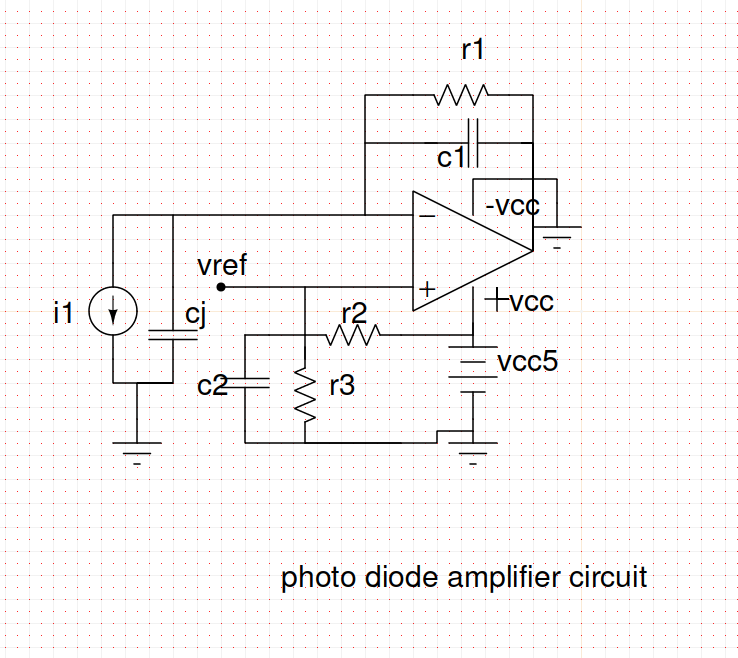
\includegraphics[scale=0.3]{photo_diode_amp.png}
\end{figure}
\newpage
\subsection{3 op-amp based Instrumentation Amplifier}
\begin{figure}[h!]
\centering
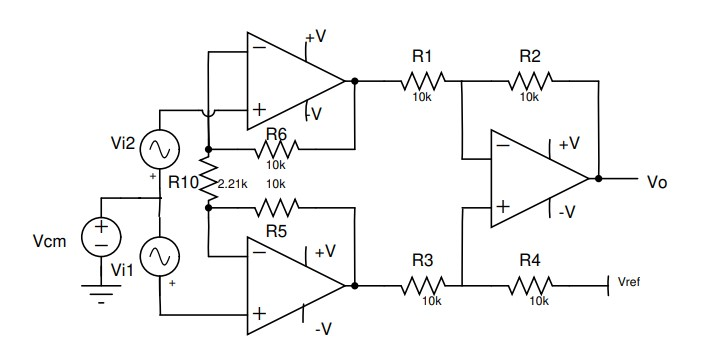
\includegraphics[scale=1]{circuit2.jpg}
\end{figure}
\newpage

\section{simulation results}
\subsection{Code Snippet}
All the files which are included in the code using .include command are already uploaded on moodle in lab submission.\\
\textbf{photo diode-current dc analysis\\}
photo diode\\
.SUBCKT LM324    1 2 3 4 5\\
C1   11 12 5.544E-12\\
C2    6  7 20.00E-12\\
DC    5 53 DX\\
DE   54  5 DX\\
DLP  90 91 DX\\
DLN  92 90 DX\\
DP    4  3 DX\\
EGND 99  0 POLY(2) (3,0) (4,0) 0 .5 .5\\
FB    7 99 POLY(5) VB VC VE VLP VLN 0 15.91E6 -20E6 20E6 20E6 -20E6\\
GA    6  0 11 12 125.7E-6\\
GCM   0  6 10 99 7.067E-9\\
IEE   3 10 DC 10.04E-6\\
HLIM 90  0 VLIM 1K\\
Q1   11  2 13 QX\\
Q2   12  1 14 QX\\
R2    6  9 100.0E3\\
RC1   4 11 7.957E3\\
RC2   4 12 7.957E3\\
RE1  13 10 2.773E3\\
RE2  14 10 2.773E3\\
REE  10 99 19.92E6\\
RO1   8  5 50\\
RO2   7 99 50\\
RP    3  4 30.31E3\\
VB    9  0 DC 0\\
VC 3 53 DC 2.100\\
VE   54  4 DC .6\\
VLIM  7  8 DC 0\\
VLP  91  0 DC 40\\
VLN   0 92 DC 40\\
.MODEL DX D(IS=800.0E-18)\\
.MODEL QX PNP(IS=800.0E-18 BF=250)\\
.ENDS\\
i 0 1 dc\\
cj 1 0 11p\\
c1 1 2 3.3p\\
r1 1 2 1.4Meg\\
vref 3 0 0.1\\
vcc1 4 0 15v\\
vcc2 5 0 -15v\\
r2 3 4 13.7k\\
r3 3 0 280\\
c2 3 0 1u\\
x1 3 1 4 5 2 LM324\\ 
.dc i 0 2.4u 0.1u\\
.control\\
run\\
plot v(2)\\ 
.endc\\
.end\\
\newpage
\textbf{photo didoe-current ac analysis\\}
photo diode\\
.SUBCKT LM324    1 2 3 4 5\\
C1   11 12 5.544E-12\\
C2    6  7 20.00E-12\\
DC    5 53 DX\\
DE   54  5 DX\\
DLP  90 91 DX\\
DLN  92 90 DX\\
DP    4  3 DX\\
EGND 99  0 POLY(2) (3,0) (4,0) 0 .5 .5\\
FB    7 99 POLY(5) VB VC VE VLP VLN 0 15.91E6 -20E6 20E6 20E6 -20E6\\
GA    6  0 11 12 125.7E-6\\
GCM   0  6 10 99 7.067E-9\\
IEE   3 10 DC 10.04E-6\\
HLIM 90  0 VLIM 1K\\
Q1   11  2 13 QX\\
Q2   12  1 14 QX\\
R2    6  9 100.0E3\\
RC1   4 11 7.957E3\\
RC2   4 12 7.957E3\\
RE1  13 10 2.773E3\\
RE2  14 10 2.773E3\\
REE  10 99 19.92E6\\
RO1   8  5 50\\
RO2   7 99 50\\
RP    3  4 30.31E3\\
VB    9  0 DC 0\\
VC 3 53 DC 2.100\\
VE   54  4 DC .6\\
VLIM  7  8 DC 0\\
VLP  91  0 DC 40\\
VLN   0 92 DC 40\\
.MODEL DX D(IS=800.0E-18)\\
.MODEL QX PNP(IS=800.0E-18 BF=250)\\
.ENDS\\
\newpage
i 0 1 dc 1.5u ac 1\\
cj 1 0 11p\\
c1 1 2 3.3p\\
r1 1 2 1.4Meg\\
vref 3 0 0.1\\
vcc1 4 0 15v\\
vcc2 5 0 -15v\\
r2 3 4 13.7k\\
r3 3 0 280\\
c2 3 0 1u\\
x1 3 1 4 5 2 LM324\\ 
.ac dec 10 10 100Meg\\ 
.control\\
run\\
plot vdb(2)\\
.endc\\
.end\\
\newpage
\textbf{instrumentation amplifier-part a}
instrumentation amplifier\\
.subckt ua741    1  2  3  4  5\\
c1   11 12 8.661E-12\\
c2    6  7 30.00E-12\\
dc    5 53 dx\\
de   54  5 dx\\
dlp  90 91 dx\\
dln  92 90 dx\\
dp    4  3 dx\\
egnd 99  0 poly(2) (3,0) (4,0) 0 .5 .5\\
fb    7 99 poly(5) vb vc ve vlp vln 0 10.61E6 -10E6 10E6 10E6 -10E6\\
ga    6  0 11 12 188.5E-6\\
gcm   0  6 10 99 5.961E-9\\
iee  10  4 dc 15.16E-6\\
hlim 90  0 vlim 1K\\
q1   11  2 13 qx\\
q2   12  1 14 qx\\
r2    6  9 100.0E3\\
rc1   3 11 5.305E3\\
rc2   3 12 5.305E3\\
re1  13 10 1.836E3\\
re2  14 10 1.836E3\\
ree  10 99 13.19E6\\
ro1   8  5 50\\
ro2   7 99 100\\
rp    3  4 18.16E3\\
vb    9  0 dc 0\\
vc    3 53 dc 1\\
ve   54  4 dc 1\\
vlim  7  8 dc 0\\
vlp  91  0 dc 40\\
vln   0 92 dc 40\\
.model dx D(Is=800.0E-18 Rs=1)\\
.model qx NPN(Is=800.0E-18 Bf=93.75)\\
.ends\\
\newpage
vcm 1 0 dc\\ 
vi1 1 2 0\\
vi2 1 4 0\\
x3 2 3 6 7 8 ua741\\
x2 4 5 9 10 11 ua741\\
r10 3 5 2.21k\\
r5 5 11 10k\\
vcc31 6 0 15v\\
vcc32 7 0 -15v\\
vcc21 9 0 15v\\
vcc22 10 0 -15v\\
r6 3 8 10k\\
r1 8 12 10k\\
r2 12 13 10k\\
r3 11 14 10k\\
r4 14 15 10k\\
vref 15 0 0\\
x1 14 12 16 17 13 ua741\\
vcc11 16 0 15v\\
vcc12 17 0 -15v\\
.dc vcm -2 2 1m\\
.control\\
run\\
plot v(13)\\
.endc\\
.end \\
\newpage
\textbf{instrumentation amplifier-part c}
instrumentation amplifier\\
.subckt ua741    1  2  3  4  5\\
c1   11 12 8.661E-12\\
c2    6  7 30.00E-12\\
dc    5 53 dx\\
de   54  5 dx\\
dlp  90 91 dx\\
dln  92 90 dx\\
dp    4  3 dx\\
egnd 99  0 poly(2) (3,0) (4,0) 0 .5 .5\\
fb    7 99 poly(5) vb vc ve vlp vln 0 10.61E6 -10E6 10E6 10E6 -10E6\\
ga    6  0 11 12 188.5E-6\\
gcm   0  6 10 99 5.961E-9\\
iee  10  4 dc 15.16E-6\\
hlim 90  0 vlim 1K\\
q1   11  2 13 qx\\
q2   12  1 14 qx\\
r2    6  9 100.0E3\\
rc1   3 11 5.305E3\\
rc2   3 12 5.305E3\\
re1  13 10 1.836E3\\
re2  14 10 1.836E3\\
ree  10 99 13.19E6\\
ro1   8  5 50\\
ro2   7 99 100\\
rp    3  4 18.16E3\\
vb    9  0 dc 0\\
vc    3 53 dc 1\\
ve   54  4 dc 1\\
vlim  7  8 dc 0\\
vlp  91  0 dc 40\\
vln   0 92 dc 40\\
.model dx D(Is=800.0E-18 Rs=1)\\
.model qx NPN(Is=800.0E-18 Bf=93.75)\\
.ends\\
\newpage
vcm 1 0 0\\
vi1 2 1 sin(0 250m 2k 0 0)\\
vi2 1 4 sin(0 250m 2k 0 0)\\
x3 2 3 6 7 8 ua741\\
x2 4 5 9 10 11 ua741\\
r10 3 5 2.21k\\
r5 5 11 10k\\
vcc31 6 0 +15v\\
vcc32 7 0 -15v\\
vcc21 9 0 +15v\\
vcc22 10 0 -15v\\
r6 3 8 10k\\
r1 8 12 10k\\
r2 12 13 10k\\
r3 11 14 10k\\
r4 14 15 10k\\
vref 15 0 0\\
x1 14 12 16 17 13 ua741\\
vcc11 16 0 15v\\
vcc12 17 0 -15v\\
.tran 0.1u 10m \\
.control\\
run\\
plot  v(2)-v(4)\\
plot  v(13)\\
.endc\\
.end \\
\newpage
\subsection{Simulation Results}
\textbf{photodiode-amplifier}
\begin{figure}[h!]
\centering
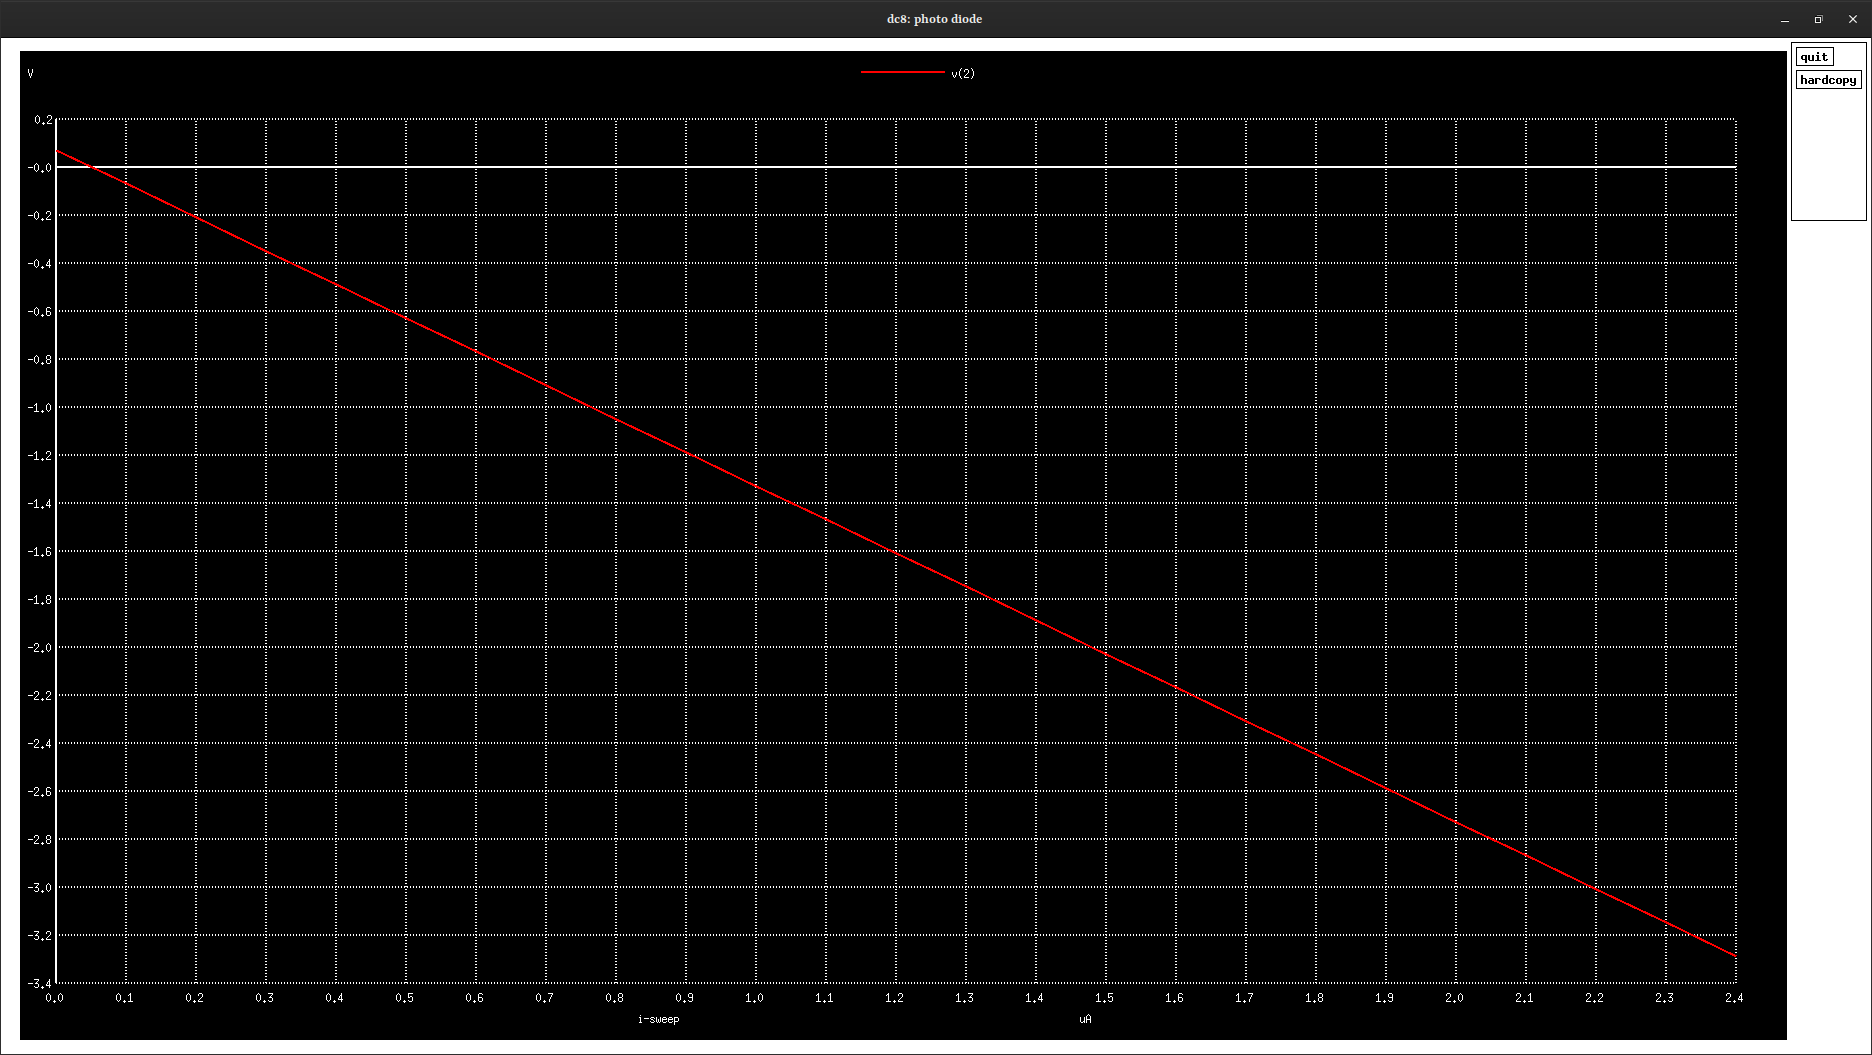
\includegraphics[scale = 0.2]{q1_a.png}
\end{figure}
\newpage
\begin{figure}[h!]
\centering
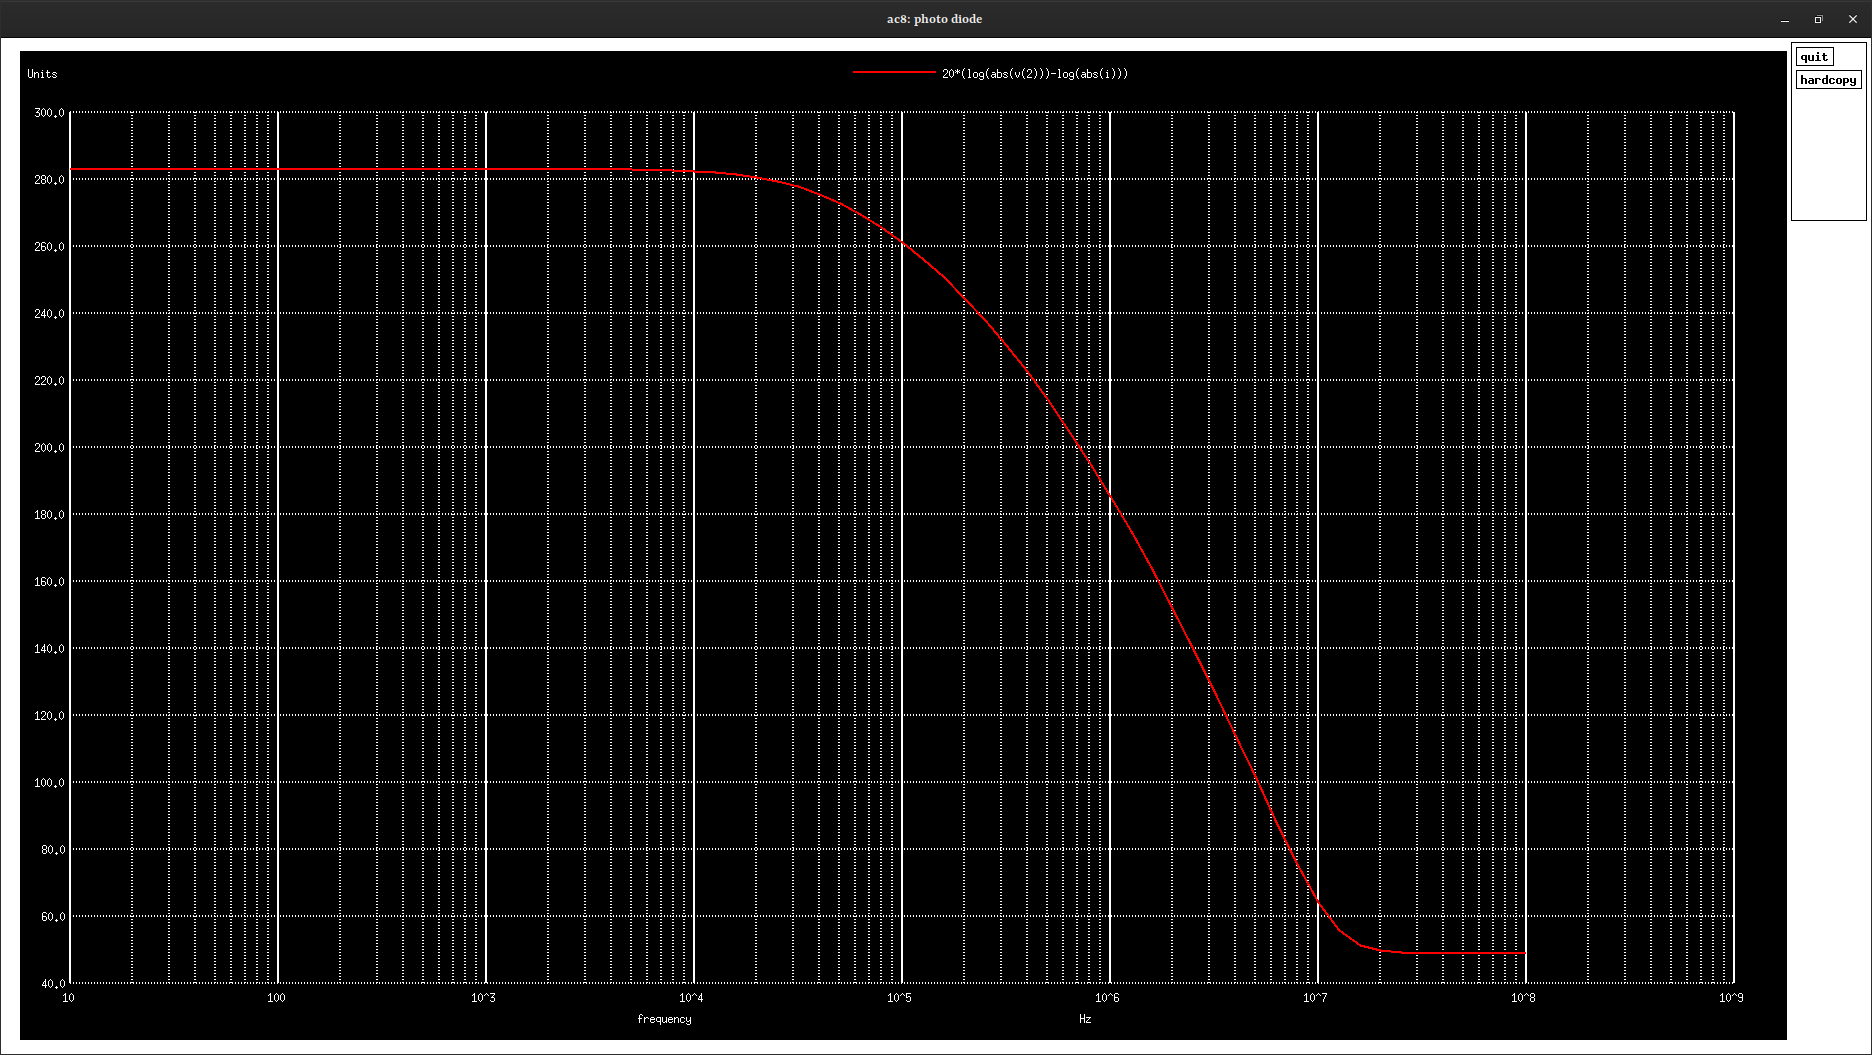
\includegraphics[scale = 0.2]{q1_b.png}
\end{figure}
The cutoff frequency for the amplifier has been calculated using the 3dB
frequency. Experimentally it came out to 580Hz\\
\newpage
\newpage
\textbf{3 op-amp based Instrumentation Amplifier\\}
\begin{figure}[h!]
\centering
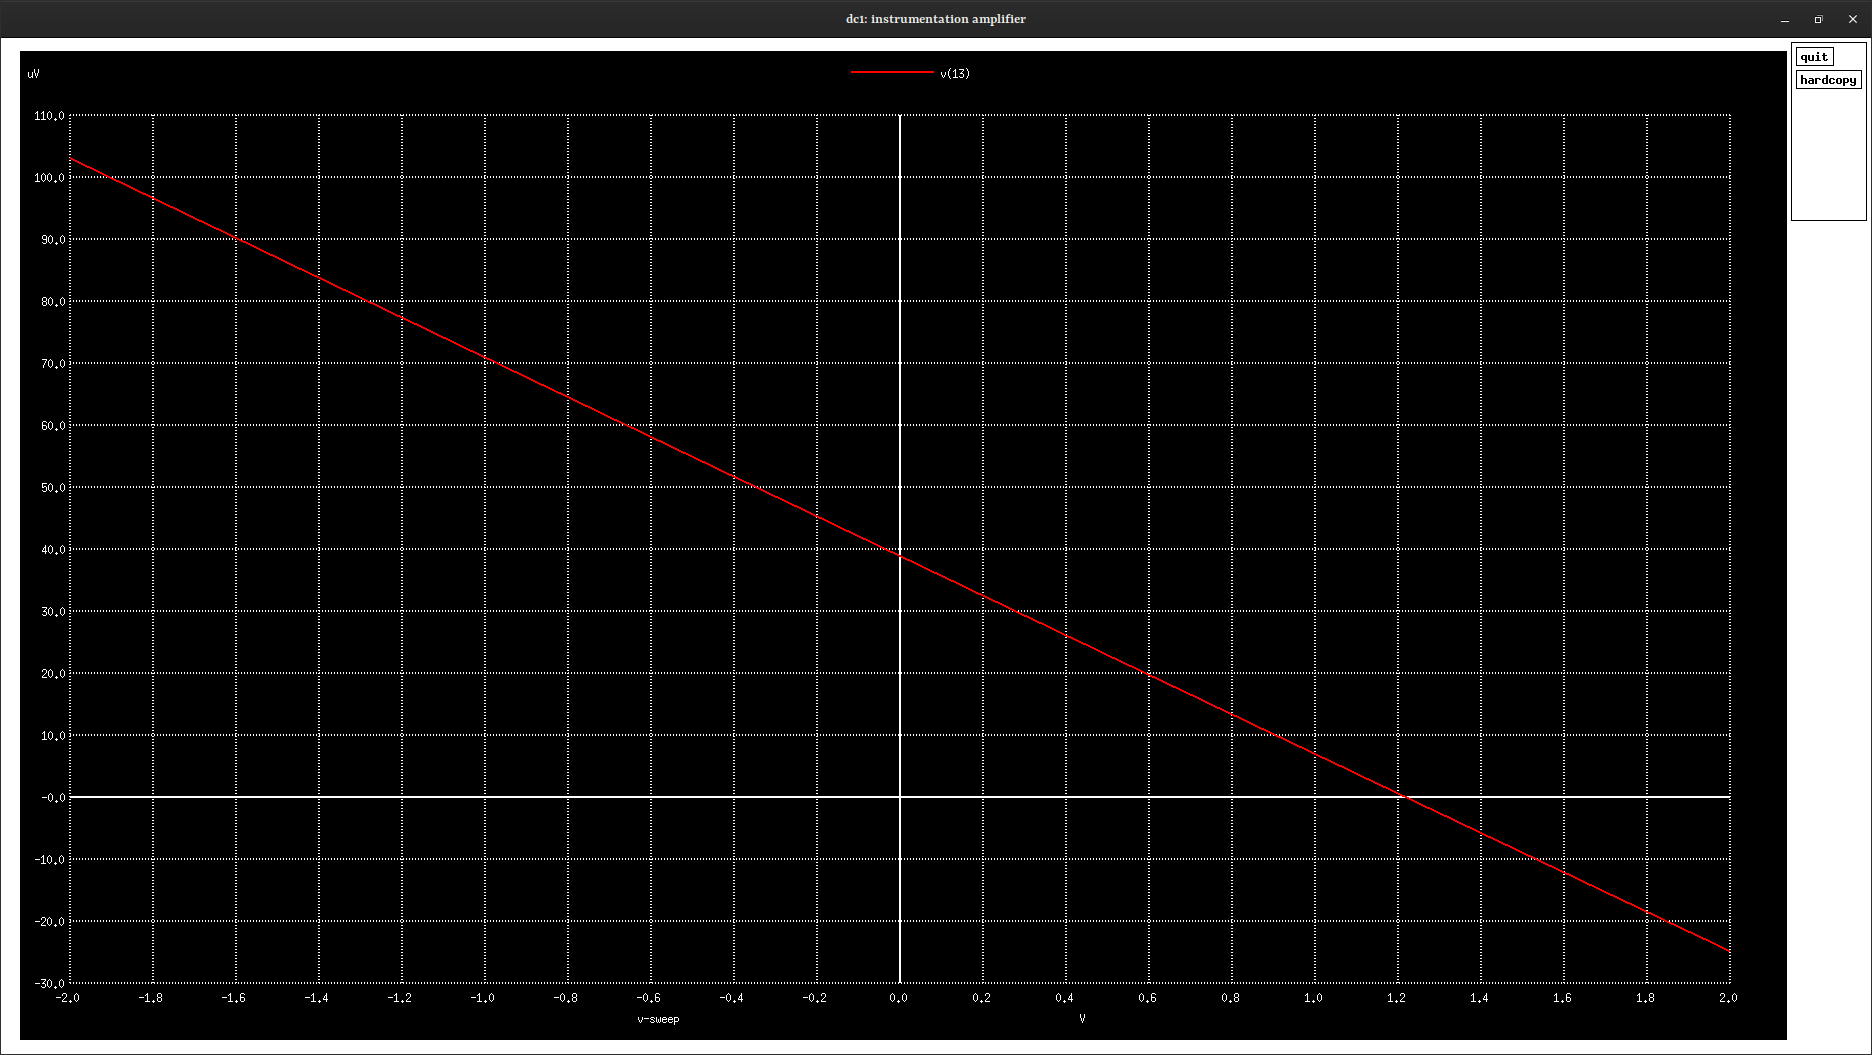
\includegraphics[scale = 0.2]{q2_a.png}
\end{figure}\\
\newpage
\begin{figure}[h!]
\centering
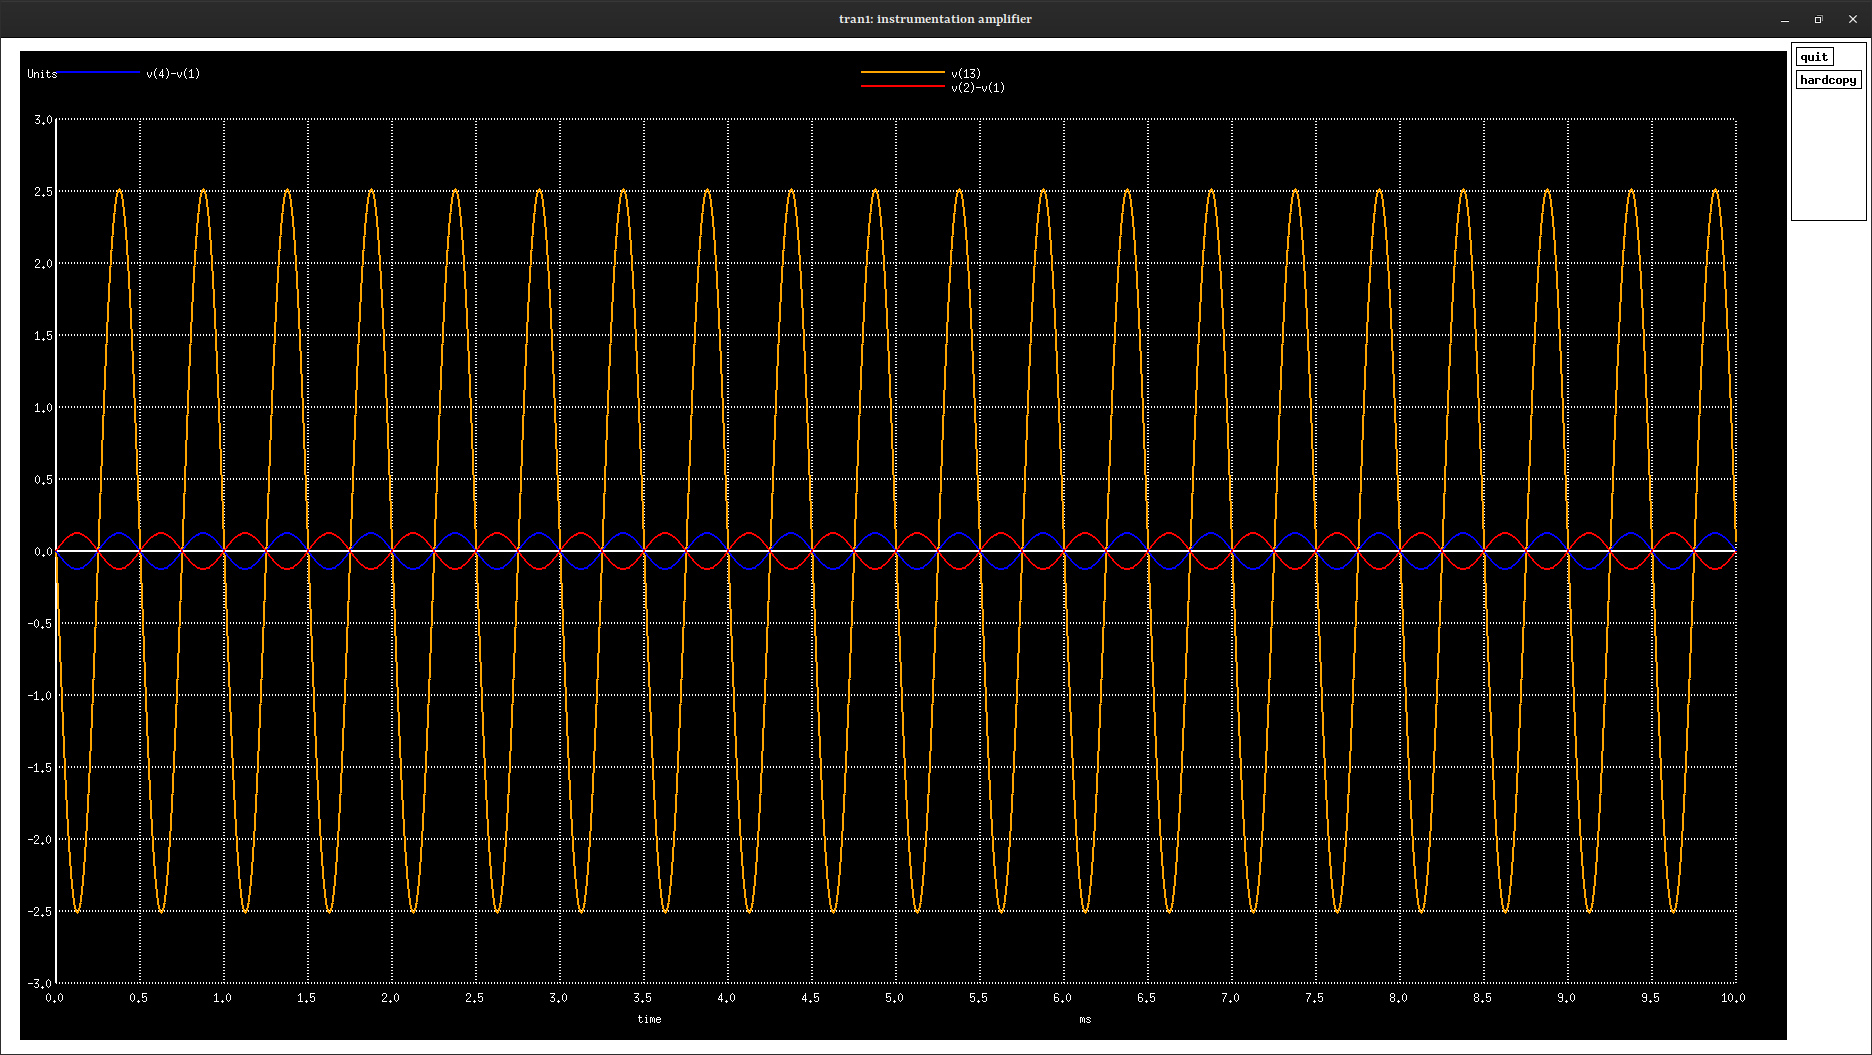
\includegraphics[scale = 0.2]{q2_c.png}
\end{figure}\\
\newpage

\begin{figure}[h!]
\centering
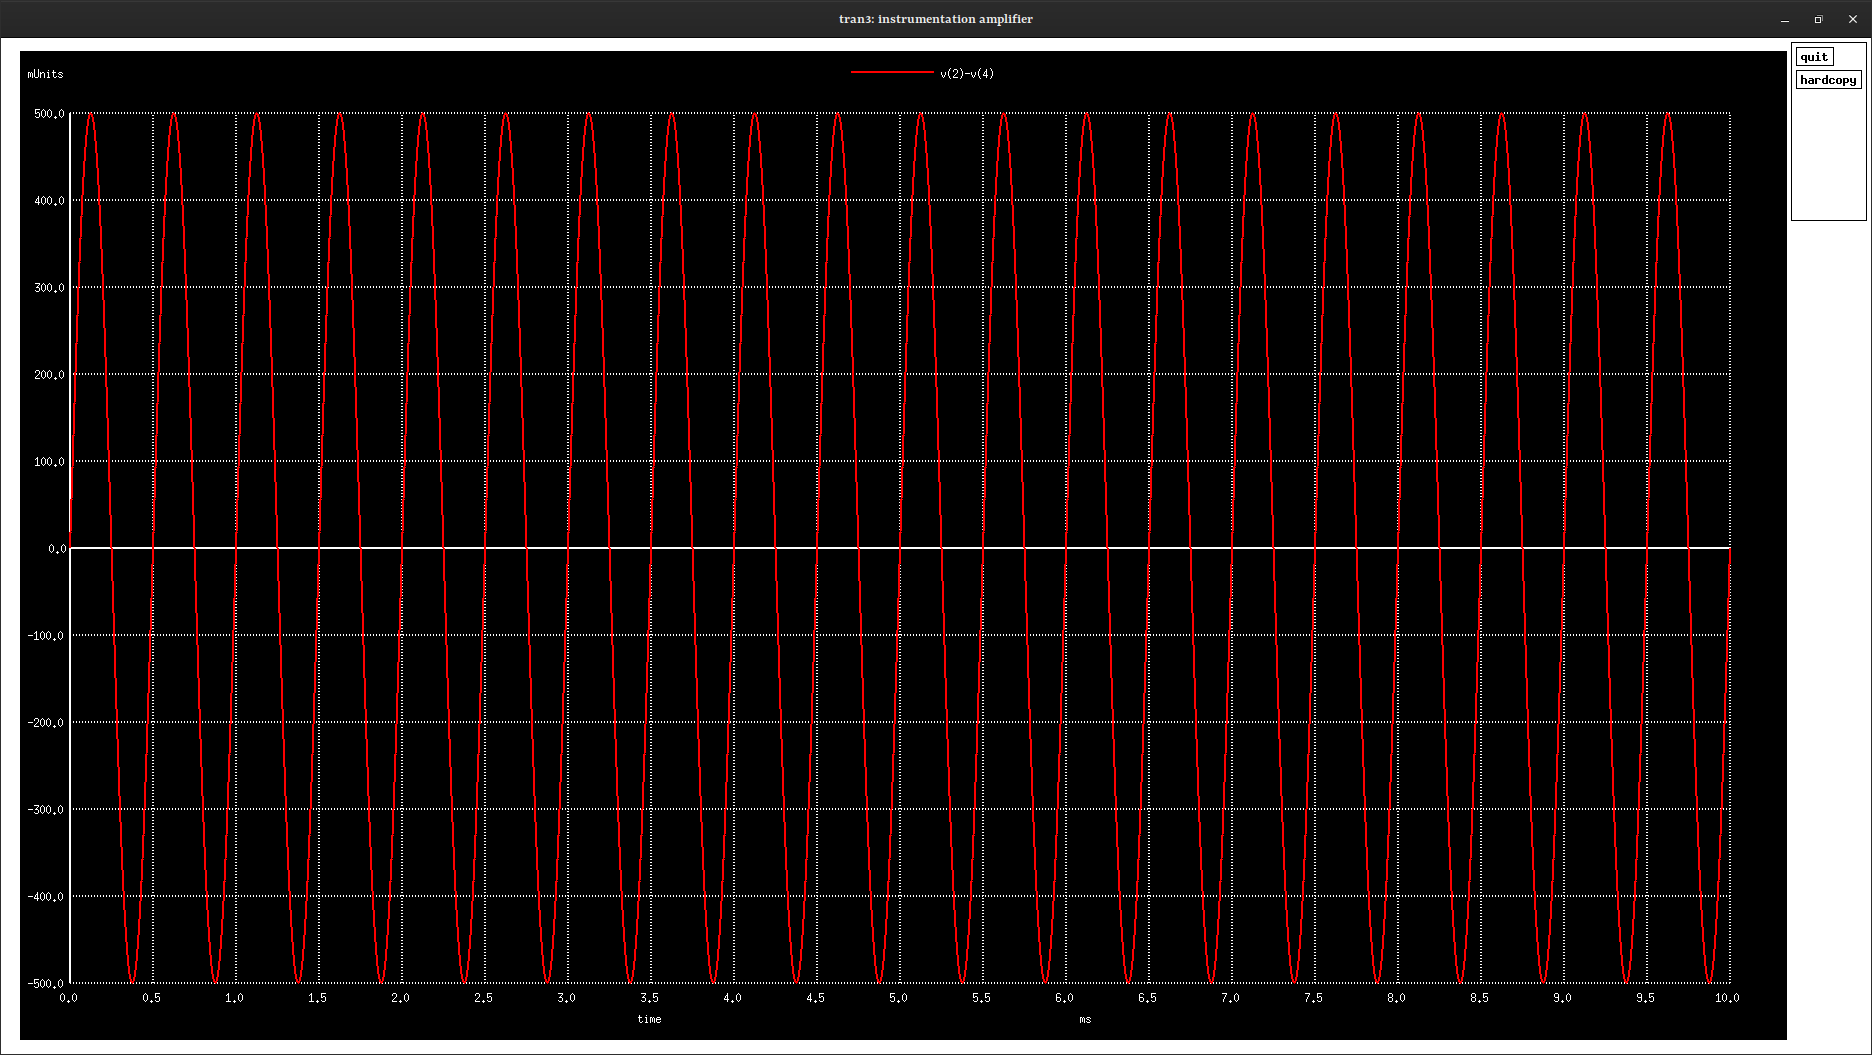
\includegraphics[scale = 0.2]{q2_c_vi1-vi2.png}
\end{figure}\\
\newpage
\begin{figure}[h!]
\centering
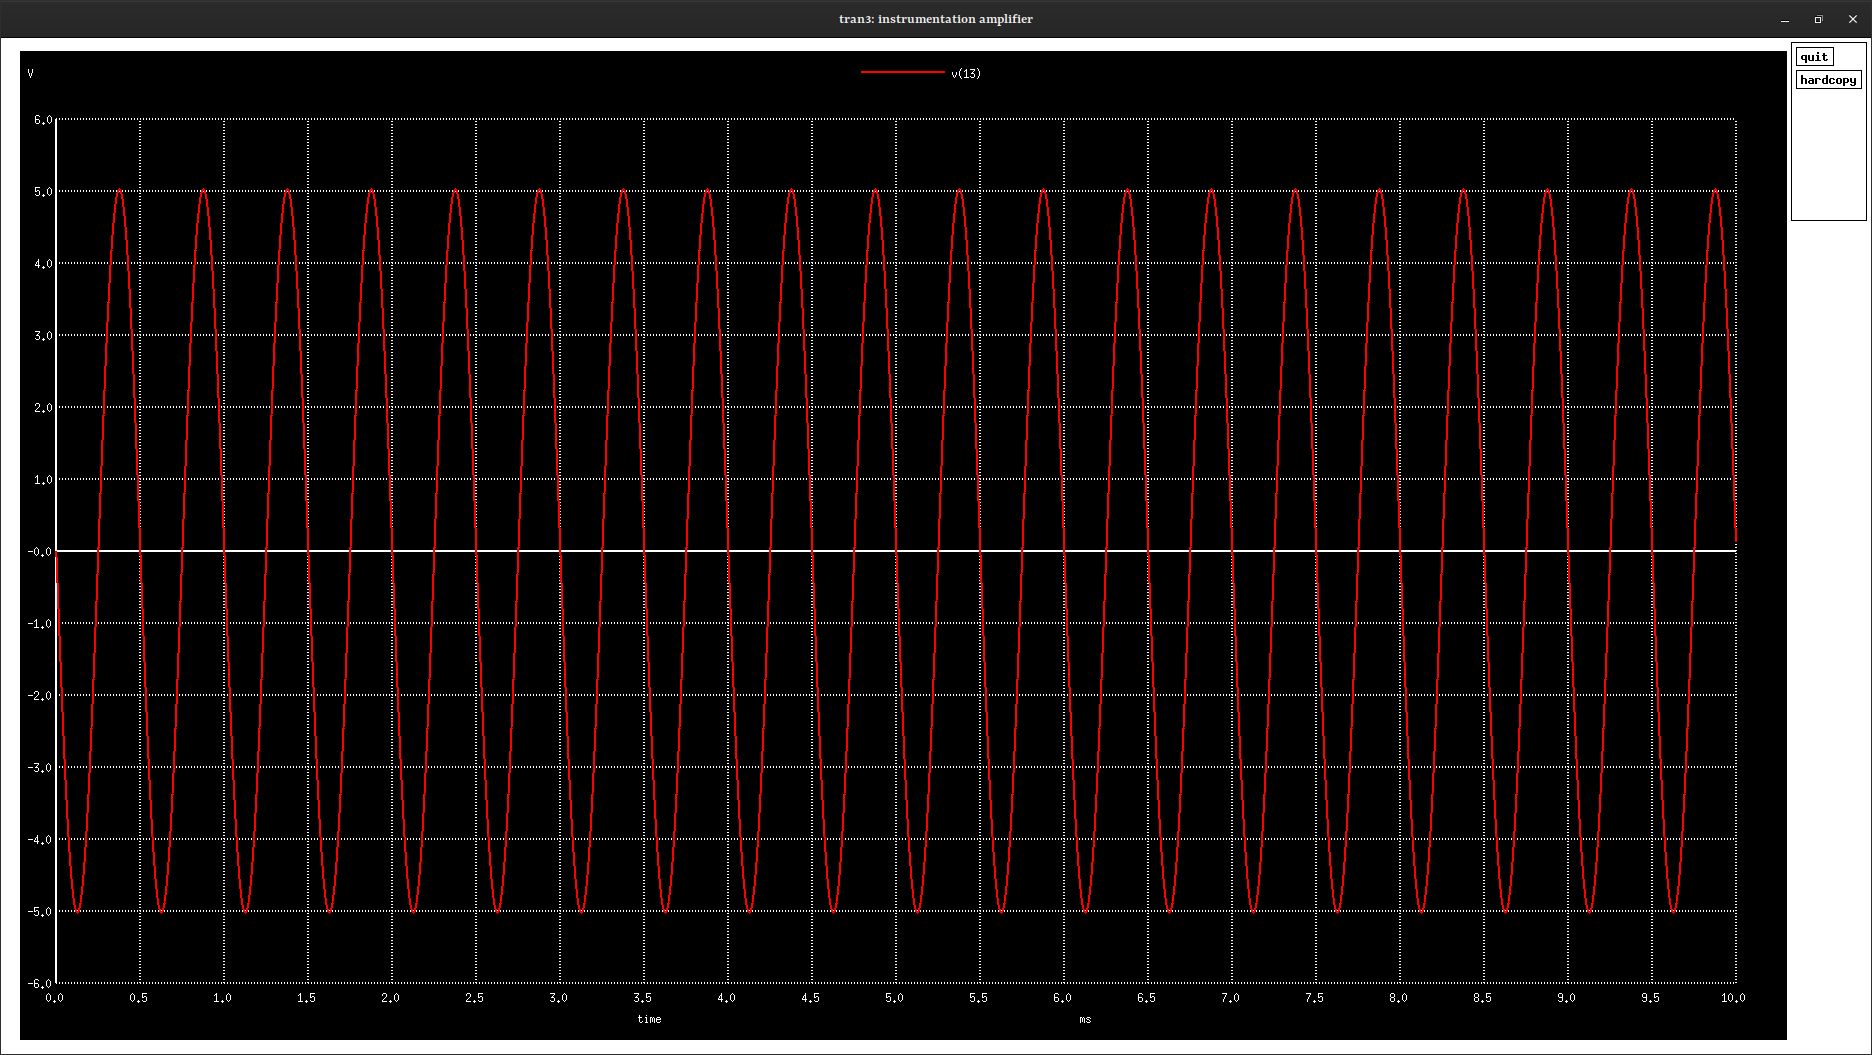
\includegraphics[scale = 0.2]{q2_c_vout.png}
\end{figure}\\
\newpage
\subsection{Explanation}
\begin{equation}
    gain=\frac{R4}{R3}*(1+\frac{2R5}{R10})
\end{equation}
differential gain came out to be 10.
\end{document}
